
\documentclass[conference]{IEEEtran}

\usepackage{amsmath}
\usepackage{caption}
\usepackage{graphicx}
\usepackage{import}
\usepackage{hyperref}
\usepackage{cleveref}
\usepackage{multicol}
\usepackage[square,sort,comma,numbers]{natbib}
\usepackage[abs]{overpic}
\usepackage{setspace}
\usepackage{subcaption}
\usepackage{morefloats}

\begin{document}
%
% paper title
% can use linebreaks \\ within to get better formatting as desired
\title{MedRadio Receiver Design}


% author names and affiliations
% use a multiple column layout for up to three different
% affiliations
\author{\IEEEauthorblockN{Elie Rosen, Gradeigh Clark, Jianqing Liu, Fanpeng Kong}
\IEEEauthorblockA{Department of Electrical and Computer Engineering\\
Rutgers, the State University of New Jersey\\
Piscataway, New Jersey 08854}}

% make the title area
\maketitle

\begin{abstract}
In this paper, we present the design of a high gain, low power, and low noise front-end Medical Device Radiocommunications Service (MedRadio) receiver for wireless medical technology applications. We employ a low-IF architecture operating at 400MHz using 0.18 um CMOS technology from the IBM7RF library. Cumulatively, we present individual designs for a low noise amplifier (LNA), a mixer, and a voltage controlled oscillator (VCO) that have been tuned to minimize power while matching to one another's design constraints. The receiver achieves 36dB gain with a 3.65dB noise figure and 1.8mW of power consumption.
\end{abstract}


\IEEEpeerreviewmaketitle

\section{Introduction}
include description of the targeted application, introduction of the problem with relevant literature review ~\cite{cha1}, ~\cite{cha2}.

\section{Receiver Architecture}

\begin{figure}[h]
   \centering
    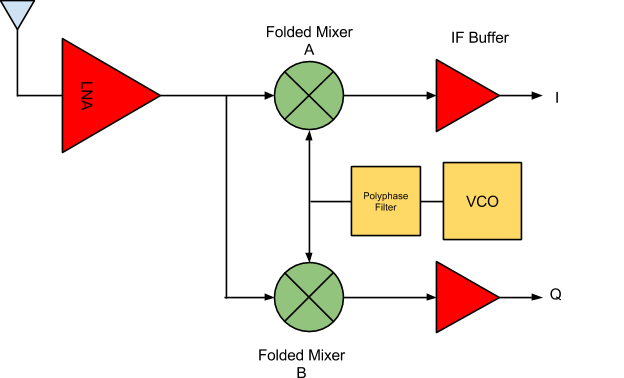
\includegraphics[width=0.55\textwidth]{figures/receiver}
    \caption{
        Block diagram of our low-IF receiver architecture. Folder mixers A and B are meant to implement quadrature downconversion. Due to time constraints, only the LNA, mixer A, and the VCO were fully implemented and integrated.
    }
    \label{fig:receiver}
\end{figure}

We considered several different architectures so as to make an informed decision as to what would be the best choice for the receiver. Our final choice was the low-IF architecture, but we will include what demotivated us towards selecting the other available ones. Primarily, we referred to Razavi~\cite{Razavi} when studying each architecture choice.


\subsection{Receiver Tradeoffs}
\subsubsection{Direct Conversion}
We have a channel bandwidth of 300 kHz in the 402-405 MHz core band and 100 kHz in the 401-402 MHz, 405-406 MHz sidebands. This channel bandwidth being downconverted directly would expose it to damaging flicker noise since CMOS technology is the primary circuit component in the LNA, filter, et cetera. Additionally, there are DC offset	 and local oscillator leakage problems that will contribute further to signal degradations.

\subsubsection{Super Regenerative}
Super regenerative receiver architectures have very good gains for the frequency range MedRadio operates at but requires a low number of interferers from neighboring bands and channels. The positive feedback architecture can serve to amplify noise to an unstable degree. As such, it suffers from poor selectivity, sensitivity (can be from 5-20 dB lower than heterodyne architectures), data rates, and has limited demodulation capability. 

\subsubsection{Dual-IF} 
Dual down conversion allows for both good channel selection and image rejection. However, multiple mixers increase the complexity of the circuit layout and requires additional band select, image reject, and channel selection components along the chain. This makes it difficult to manage reasonable linearity with good noise, power dissipation, and gain. So this won’t work for our application either. Also,  we want to avoid as many mixing spurs as possible and multiple image problems.

\subsubsection{Zero-Second IF}
This fixes the secondary image problem from Dual-IF but doesn’t fix the other issues. Additionally, it operates in the baseband -- where the flicker noise is the highest! This is unfeasible for us.

\subsection{Target Architecture: Low-IF}
Low-IF is an optimal choice for this type of application. The spectrum can be downconverted to a point where the Q factor is much lower and circuits can be designed using lower, optimal values. Downconverting the signal to a low frequency that isn't inside of the baseband (as in zero-IF) can help to avoid degradation from flicker noise of the MOSFETs.  Additionally, there is better frequency isolation in this architecture because the IF frequency can be selected such that the difference between the local oscillator (LO) frequency and the RF frequency is quite small. 

The downsides to this selection is that there are tradeoffs betwen image rejection and channel selection. High-IF implementations causes substantial image rejection since the image would be far outside of the bandwidth of the image-reject filter. However, this allows for close-by interferers to be allowed in with the spectrum of interest. Similarly, low-IF implementations cause substantial channel rejection by narrowly selecting the spectrum but allowing in images that are nearby to be downconverted to the same point. This issue, however,  can be fixed by implementing quadrature downconversion after the mixer.
\section{Circuit Design}
include three sub-sections: one for LNA, one for Mixer and one for VCO. For each subsection discuss the design procedure (describe the circuit architecture, provide justification, and describe your approach for determining the size of transistors and the values of passive elements), include transistor-level schematic, simulation results, and a table summarizing the performance metrics of the circuit.

\subsection{Low Noise Amplifier}

\subsection{Mixer}

\subsection{Voltage Controlled Oscillator}
As shown in Figure /ref{vco}, the proposed single-ended VCO uses a pair of complementary np-MOSFETs so that the dc current can be reused and a low power VCO can be realized [1]. The LC tank will determine the oscillation frequency by:

f_0 = 1 / 2pi sqrt(L_2 C_v)

Note that, Cv includes varactors, gate-source and drain-source capacitors of np-MOSFETs. The varactors are used to tune the VCO oscillation frequency. And on the other hand, the transistors are configured to provide a negative resistance to compensate the tank loss. 

FIGURE HERE

The nMOS has the dimension of $L/W=0.18/30$ and the pMOS has the dimension of $L/W=0.18/200$, both in m. The values for inductor and varactors are optimized to center the oscillation frequency at 400 MHz. Note that, for better estimation of the VCO performance, all the capacitors, inductors and resistors are used as non-ideal components in the Cadence simulation. 


\section{Results}
\subsection{Low Noise Amplifier}
Fig. ~\ref{fig:s11} shows the S11 parameters of the LNA, which indicates the input matching quality. The minimum input matching is -21 dB. Fig. ~\ref{fig:s22}, the S22, output matching is presented. The minimum matching point is -22 dB. Also, the gain (S21 parameters) can be seen from Fig. ~\ref{fig:s21}. This LNA provides a relative high gain, 17.5 dB. To show the linearity property of the LNA, the 1 dB compression point plot is presented in Fig. ~\ref{fig:lnaiip3}. From the figure, the 1 dB compression point is ??. Also, the IP3 is done by cadence simulation, which is shown in Fig. ~\ref{fig:1db}. The IP3 point is. What is more, noise figure should be presented to analysis the LNA. In Fig. ~\ref{fig:lnanoise} and Fig. ~\ref{fig:lnanoisemin}, we display the noise figure and minimum noise figure of the proposed LNA. The noise figure is 3.4 dB and the minimum noise figure is 1.2 dB. To match the design requirement, the DC power consumption of the LNA is 0.57 mW. 

%s11
\begin{figure}[h]
   \centering
    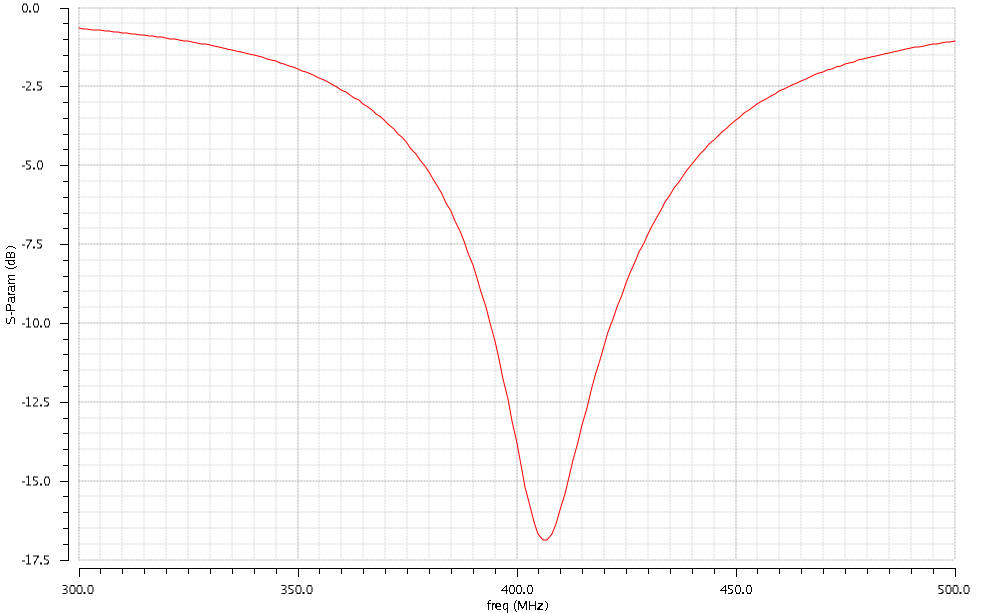
\includegraphics[width=0.5\textwidth]{figures/s11.png}
    \caption{Graph of LNA S11 input matching}
    \label{fig:s11}
\end{figure}

%s22
\begin{figure}[h]
   \centering
    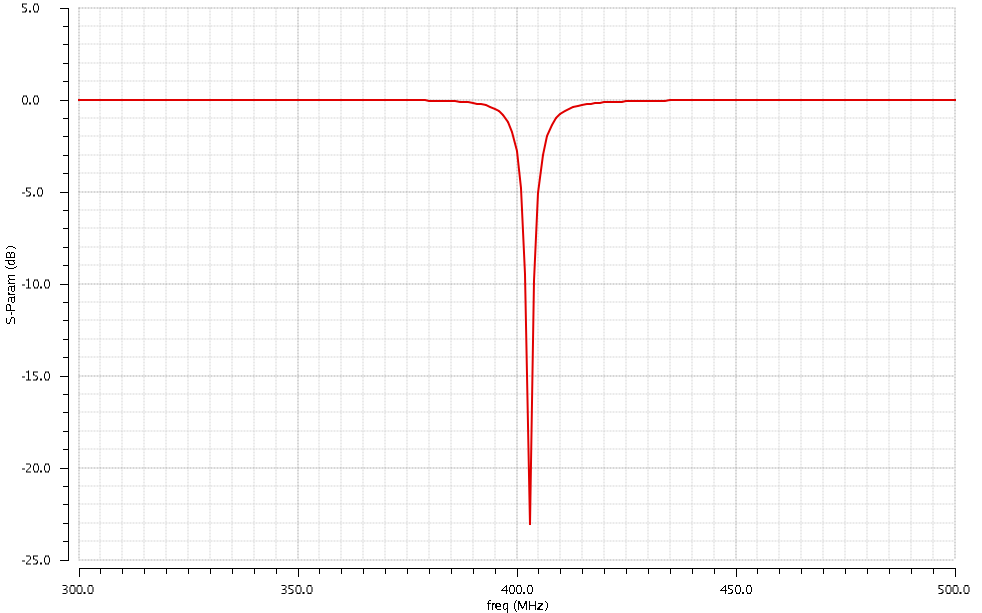
\includegraphics[width=0.5\textwidth]{figures/s22.png}
    \caption{Graph of LNA S22 output matching}
    \label{fig:s22}
\end{figure}

%s21
\begin{figure}[h]
   \centering
    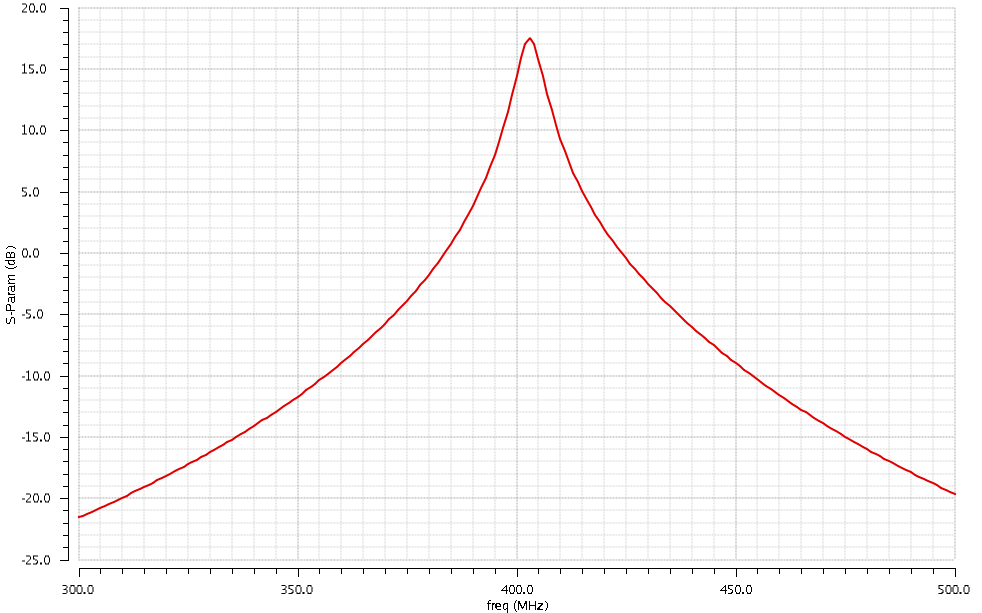
\includegraphics[width=0.5\textwidth]{figures/s21.png}
    \caption{Graph of LNA S21 gain}
    \label{fig:s21}
\end{figure}

%1dbcompression
\begin{figure}[h]
   \centering
    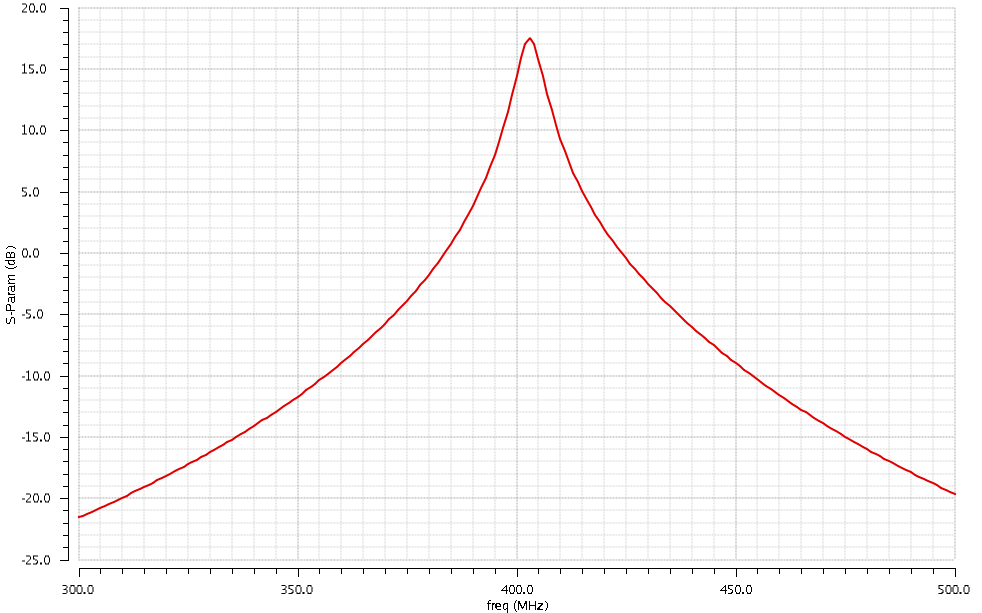
\includegraphics[width=0.5\textwidth]{figures/s21.png}
    \caption{LNA 1 dB compression point}
    \label{fig:1db}
\end{figure}

%IIP3
\begin{figure}[h]
   \centering
    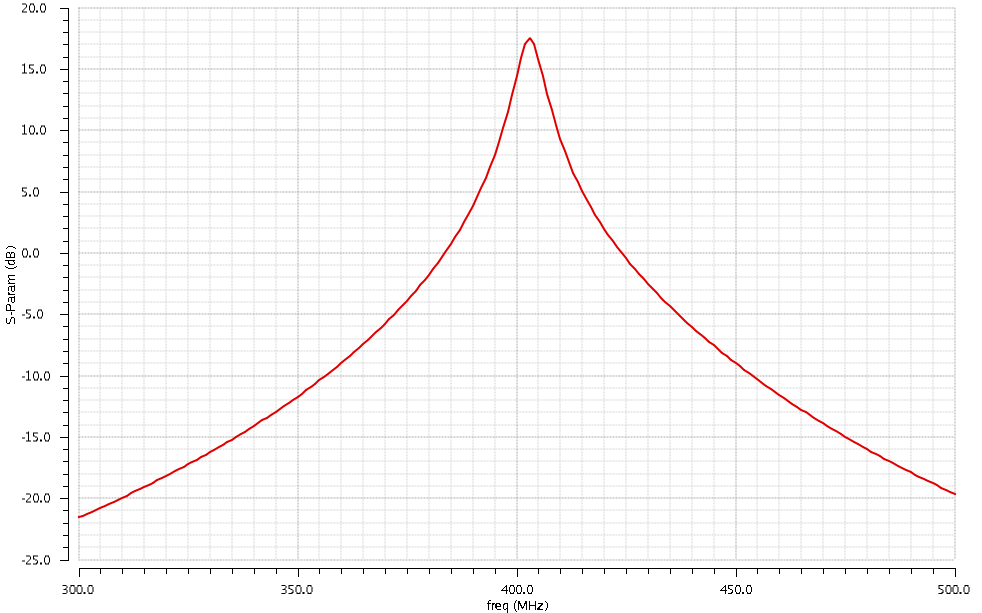
\includegraphics[width=0.5\textwidth]{figures/s21.png}
    \caption{LNA Linearity}
    \label{fig:lnaiip3}
\end{figure}

%noise
\begin{figure}[h]
   \centering
    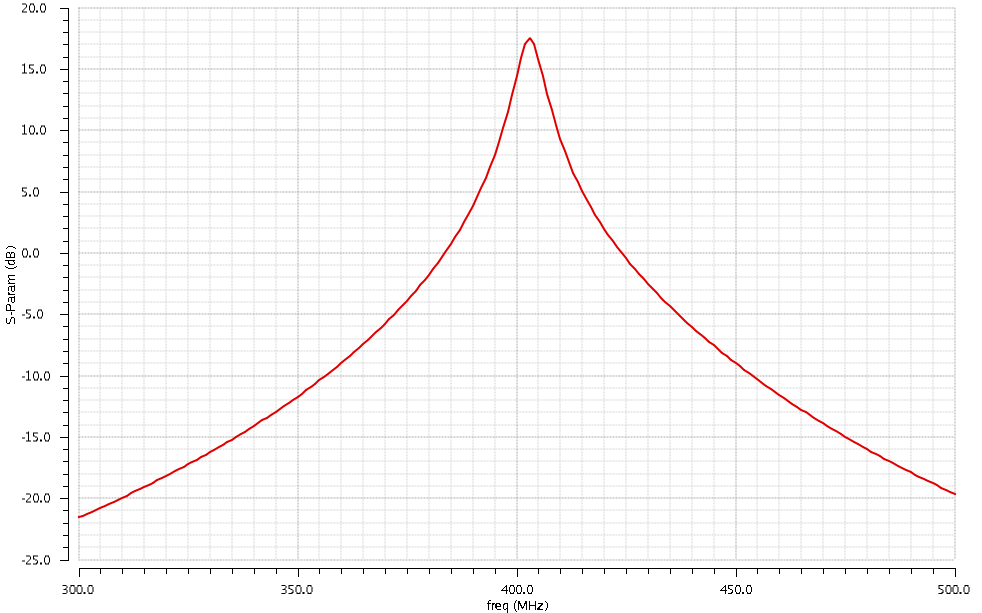
\includegraphics[width=0.5\textwidth]{figures/s21.png}
    \caption{Graph of LNA noise figure}
    \label{fig:lnanoise}
\end{figure}

%min noise
\begin{figure}[h]
   \centering
    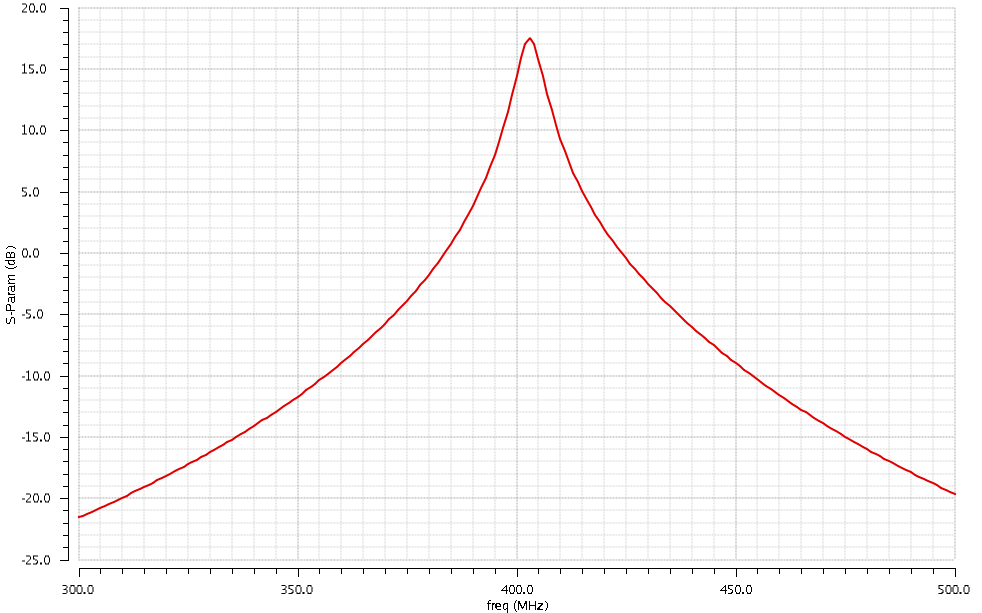
\includegraphics[width=0.5\textwidth]{figures/s21.png}
    \caption{Graph of LNA minimum noise figure}
    \label{fig:lnanoisemin}
\end{figure}

\subsection{Mixer}
Although the assignment only asked to see conversion gain with respect to frequency as shown in Fig. ~\ref{fig:cgfreq} we also simulated for conversion gain with respect to input power as shown in Fig. ~\ref{fig:cgpwr}. These graphs show that the mixer is able to maintain good gain across the frequencies of interest as well as consistent gain across sensitivities as low as -100 dBm. Fig. ~\ref{fig:loif} and Fig. ~\ref{fig:lorf} show the VCO feedthrough to the input and output ports. As can be seen in the graphs, the setup of the mixer causes this these figures to be very low. The noise of the mixer was found to be 4.40 dB as shown in Fig. ~\ref{fig:mixernoise}. Lastly, the linearity of the mixer can be found in Fig. ~\ref{fig:mixerlin}. The linearity is quite lower than expected however this was a trade-off to achieve a high gain and low noise. Final mixer results can be found in TABLE ~\ref{tab:mixerresults}.

%table of results
\begin{table}[h]
\begin{center}
	\begin{tabular}{ |c | c | }
 		\hline                      
  		Conversion gain &  10.50 dB\\ \hline
  		LO-IF feedthrough &  -75.06 dB\\ \hline
  		LO-RF feedthrough & -103.40 dB\\ \hline
		Noise Figure &  4.40 dB\\ \hline
		IIP3 & -13.26 dBm\\ \hline
		Power & 0.8 mW \\ 
  		\hline  
	\end{tabular}

\end{center}
\caption{Final results from Mixer simulations}
\label{tab:mixerresults}
\end{table}

%mixer conversion gain vs frequency
\begin{figure}[h]
   \centering
    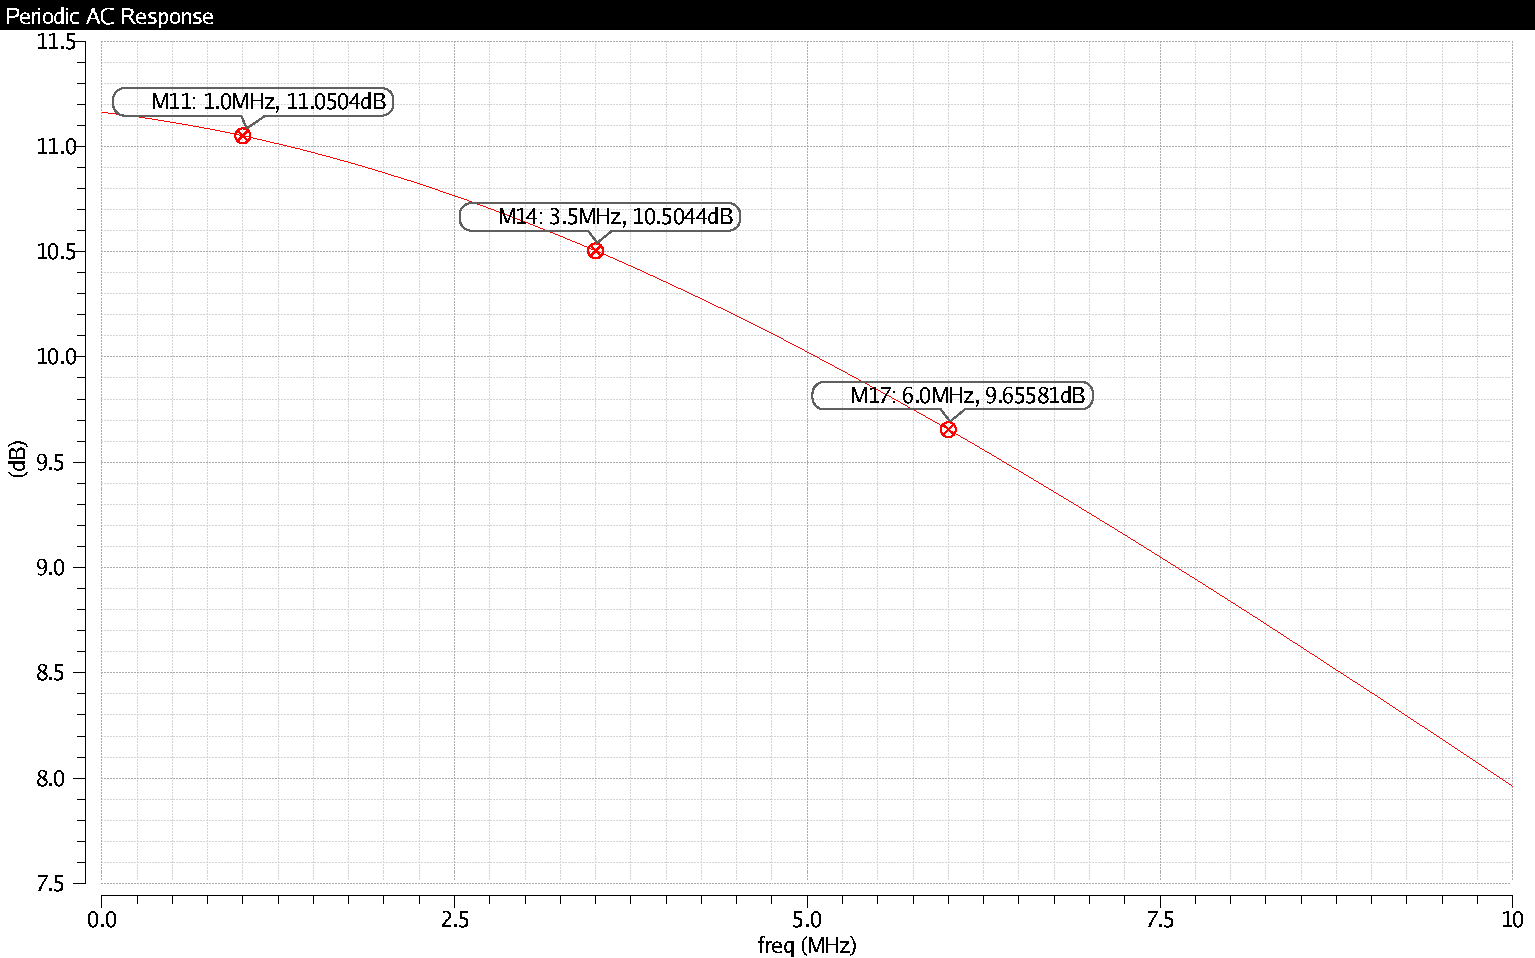
\includegraphics[width=0.5\textwidth]{figures/MixerConversionGainFreq.pdf}
    \caption{Mixer conversion gain with respect to frequency}
    \label{fig:cgfreq}
\end{figure}

%mixer conversion gain vs power
\begin{figure}[h]
   \centering
    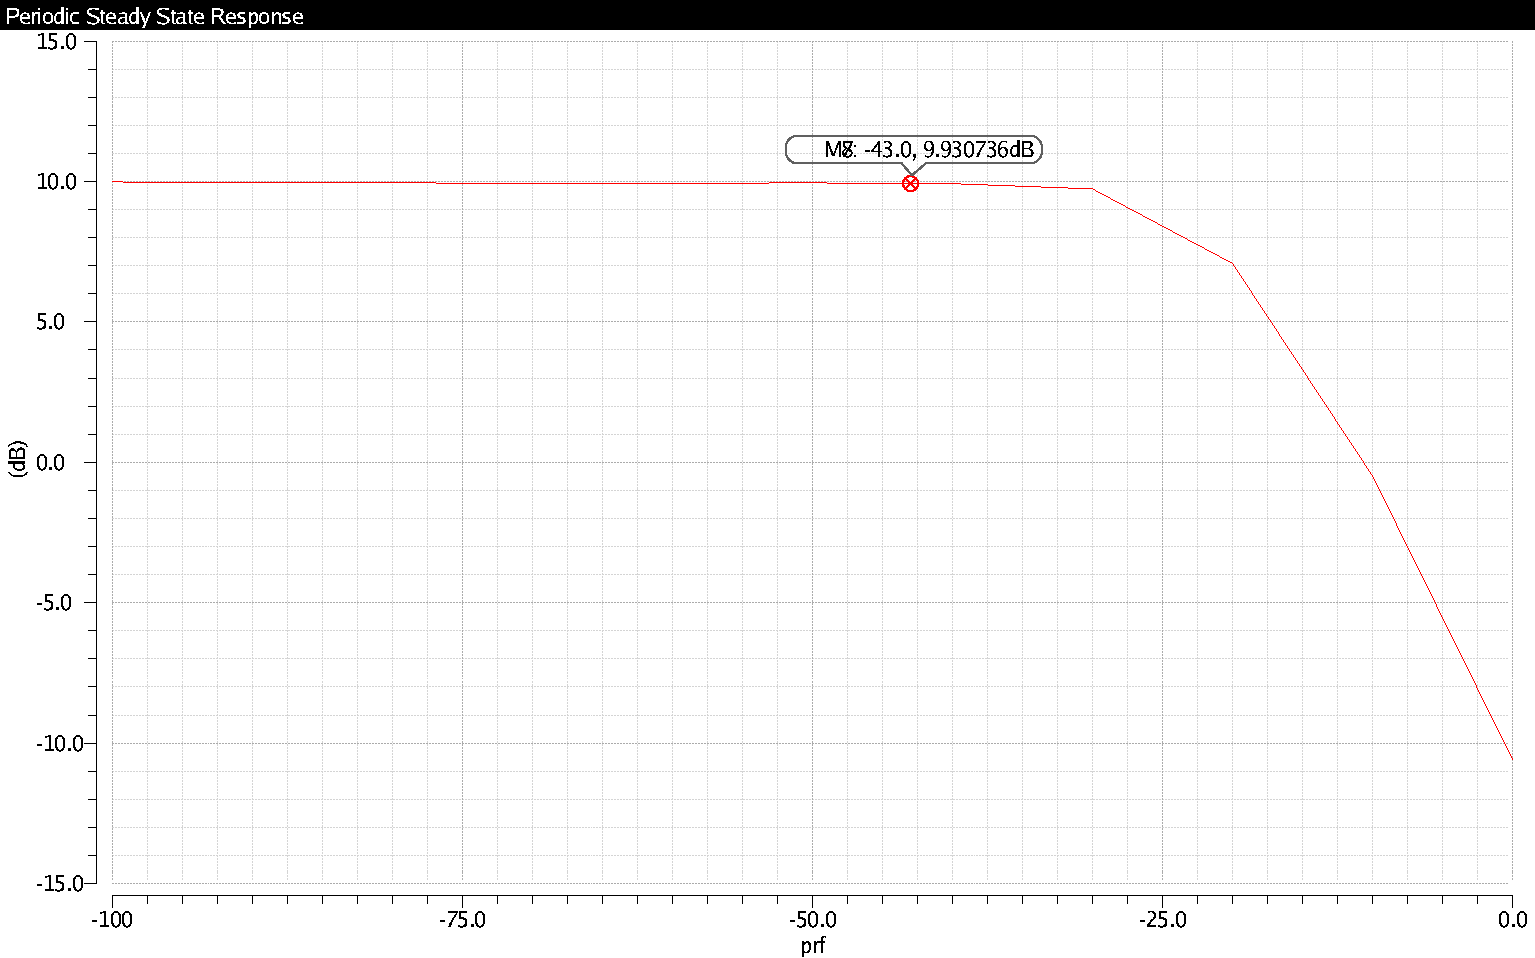
\includegraphics[width=0.5\textwidth]{figures/MixerConversionGain.pdf}
    \caption{Mixer conversion gain with respect to input power}
    \label{fig:cgpwr}
\end{figure}


%LO-IF feedthrough
\begin{figure}[h]
   \centering
    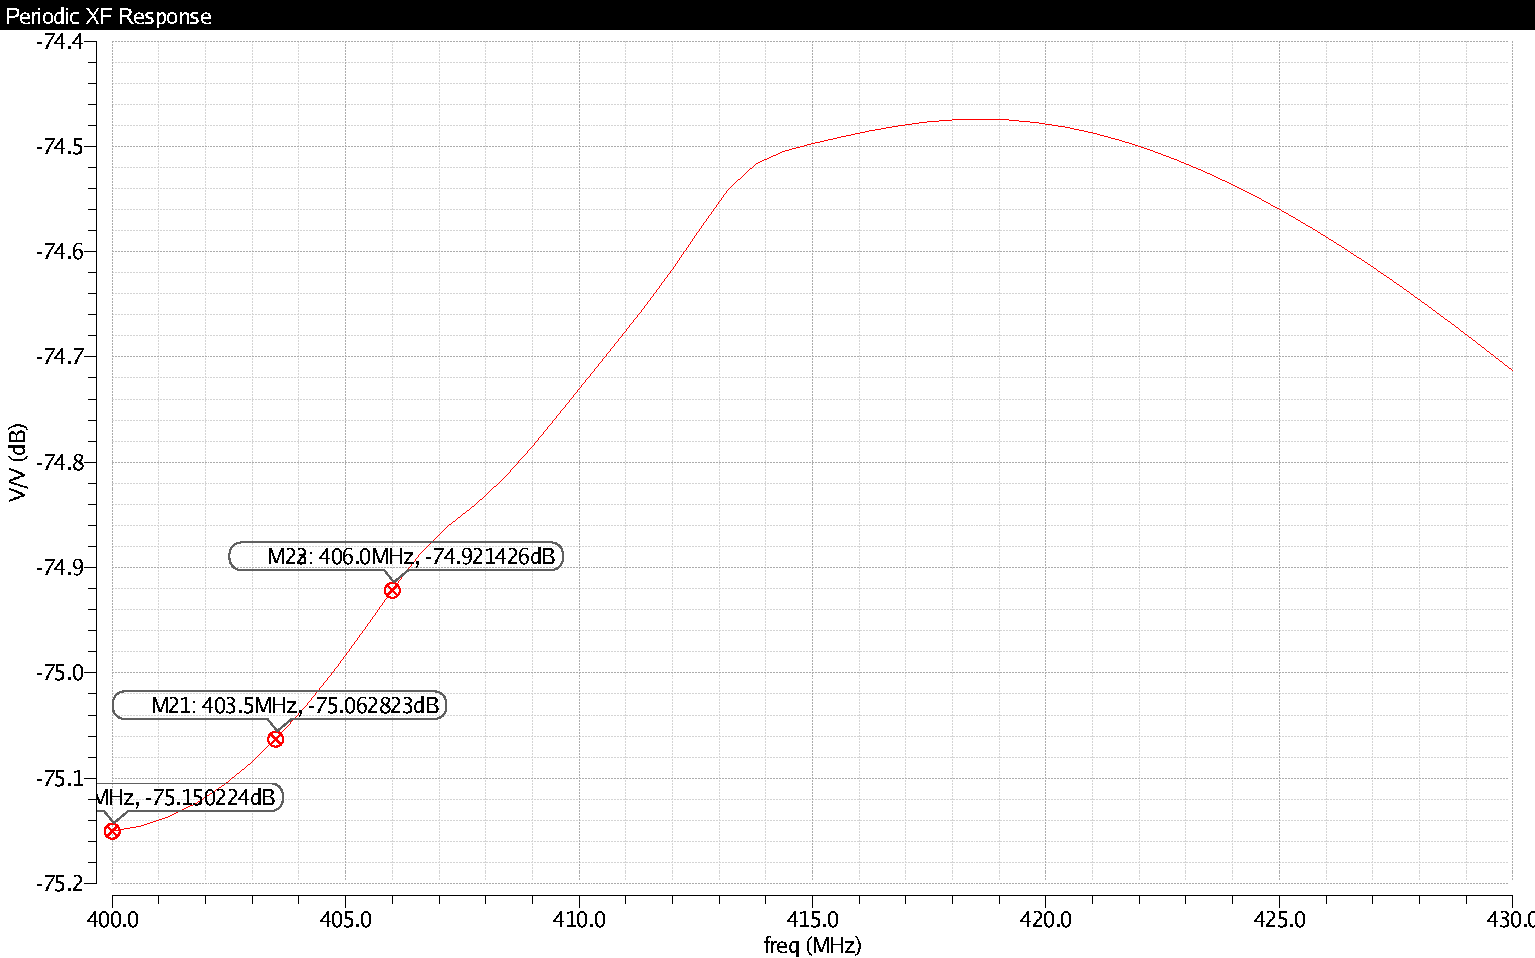
\includegraphics[width=0.5\textwidth]{figures/MixerLO-IFfeed.pdf}
    \caption{Mixer oscillator to IF output feedthrough}
    \label{fig:loif}
\end{figure}

%LO-RF feedthrough
\begin{figure}[h]
   \centering
    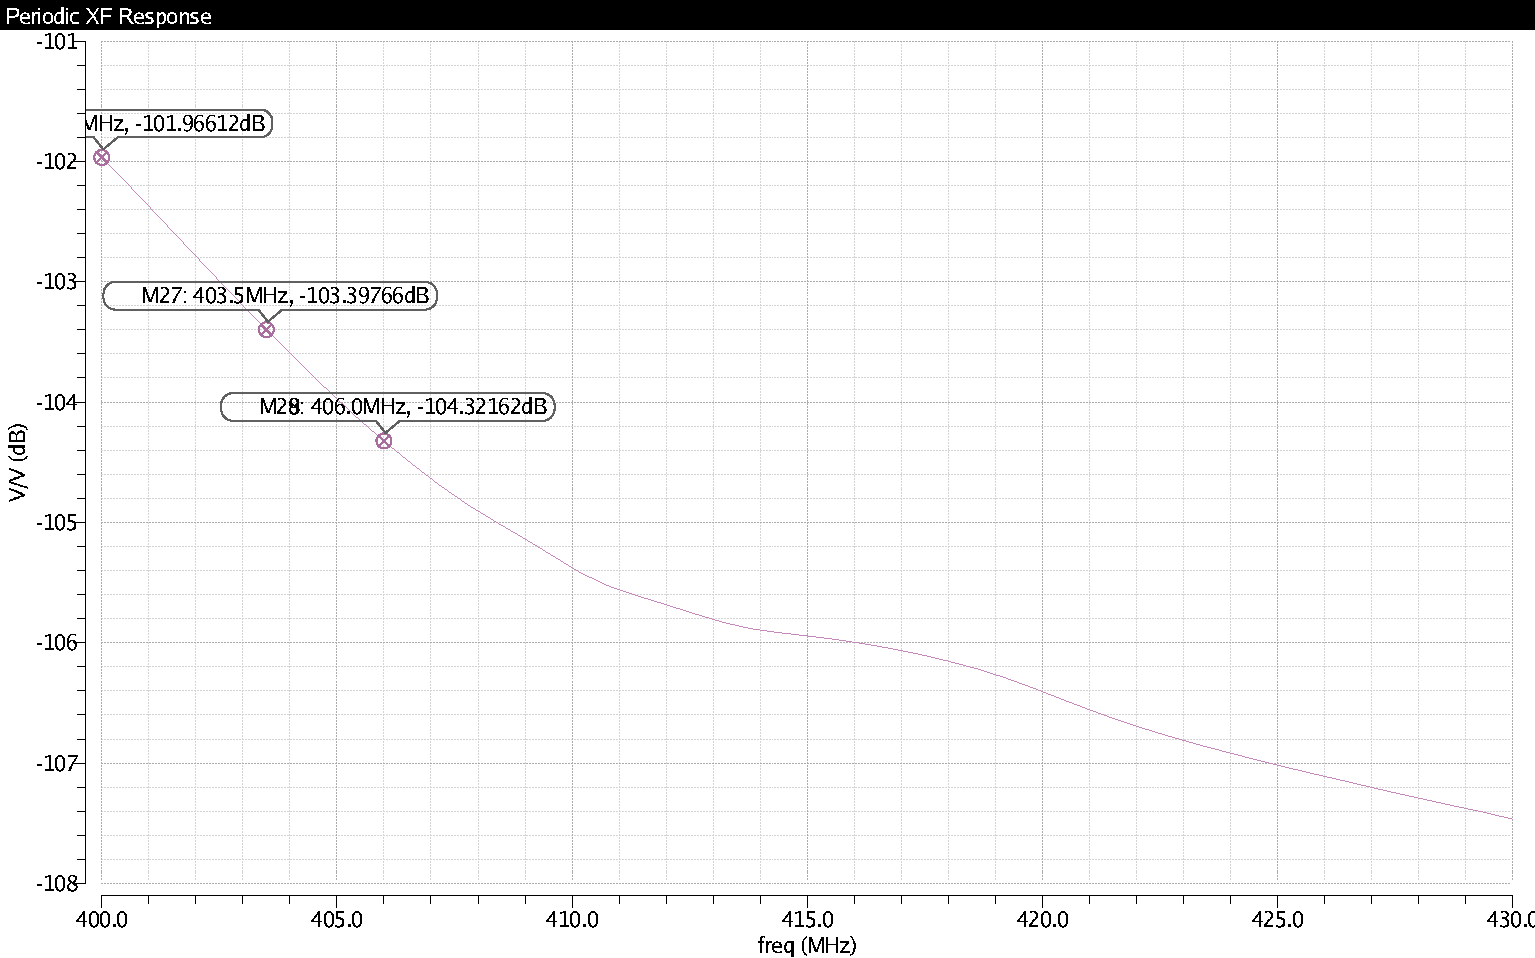
\includegraphics[width=0.5\textwidth]{figures/MixerLO-RFfeed.pdf}
    \caption{Mixer oscillator to RF input feedthrough}
    \label{fig:lorf}
\end{figure}

%Noise figure
\begin{figure}[h]
   \centering
    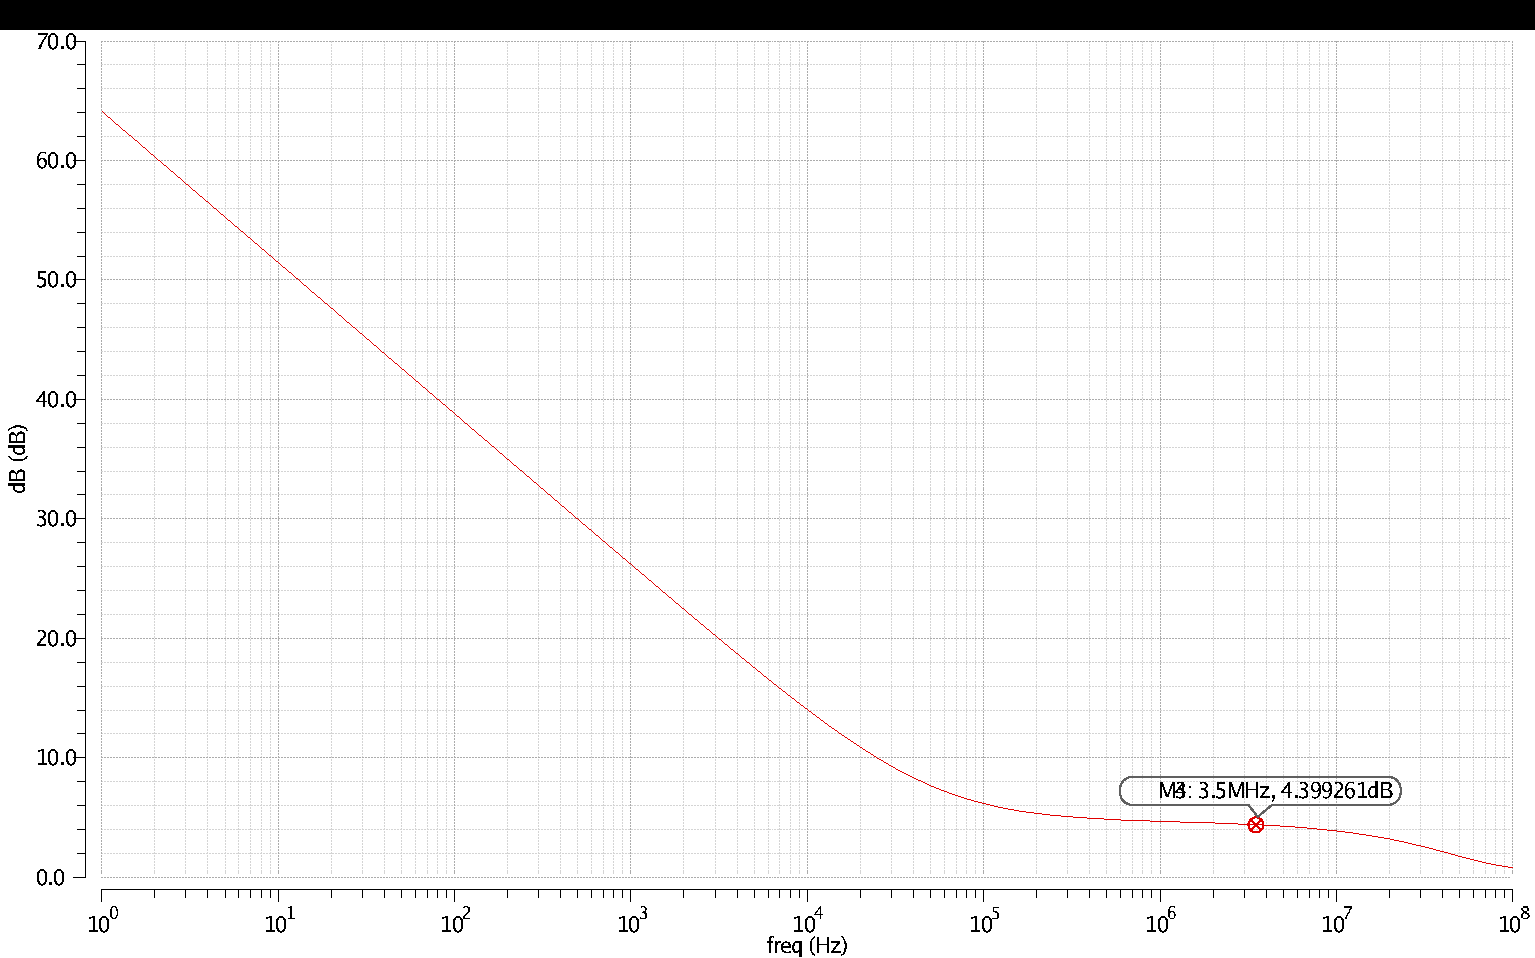
\includegraphics[width=0.5\textwidth]{figures/MixerNoiseFigure.pdf}
    \caption{Graph of Mixer Noise Figure}
    \label{fig:mixernoise}
\end{figure}

%Linearity
\begin{figure}[h]
   \centering
    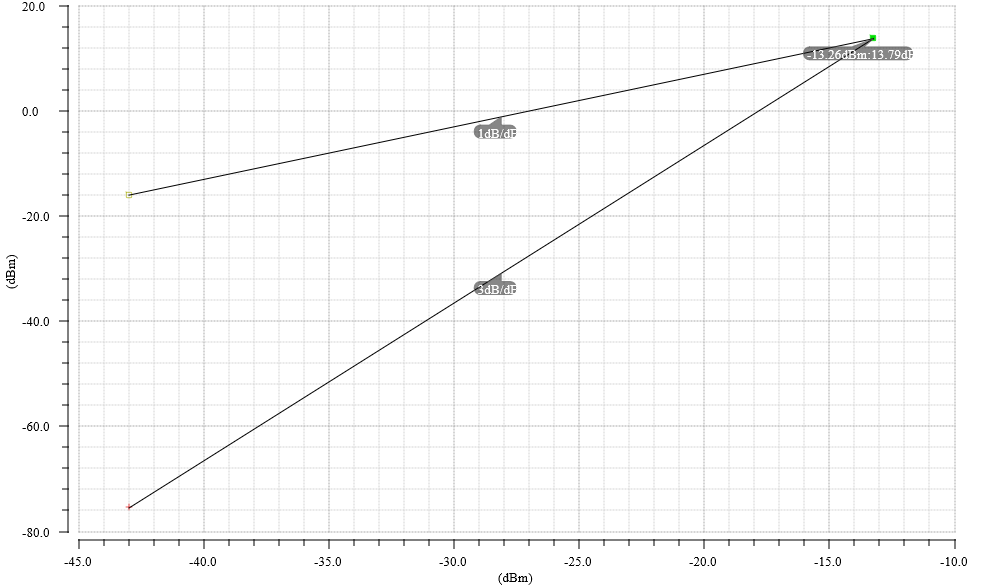
\includegraphics[width=0.5\textwidth]{figures/mixerIIP3.png}
    \caption{Graph of Mixer linearity}
    \label{fig:mixerlin}
\end{figure}

\subsection{Voltage Controlled Oscillator}
Fig.2 shows the simulated output transients of the proposed VCO; the VCO provides two differential outputs with the same peak-peak value of 305 mV. The oscillation frequency can also be calculated from the period of sinusoidal waveform, which is 400 MHz. The phase noise is shown in Fig.3 and it is -119 dBc/Hz at 1MHz offset from the center frequency of 400 MHz. Fig.4 plots the simulated tuning curve by varying the controllable voltage. As the tuning voltage sweeps from -0.5 V to 1 V, the oscillation frequency changes from 393 MHz to 400 MHz, indicating a tunable range of 6 MHz. The VCO’s power consumption, which is a critical consideration in Medradio application, is 0.2 mW.
\section{System Integration}

Since it was known ahead of time that the receiver was to be fully integrated together, a lot of effort was put towards perfecting input and output matching to guarantee maximum power transfer across components. The LNA input, VCO output, and Mixer output are all matched to 50 $\Omega$. The LNA output and Mixer signal input are matched to 500 $\Omega$, we found this to help improve the gain of the Mixer. Since all of the components were matched properly, full system integration was as simple as placing the components together (Fig.~\ref{fig:fullsystem}). 

\begin{figure}[H]
   \centering
    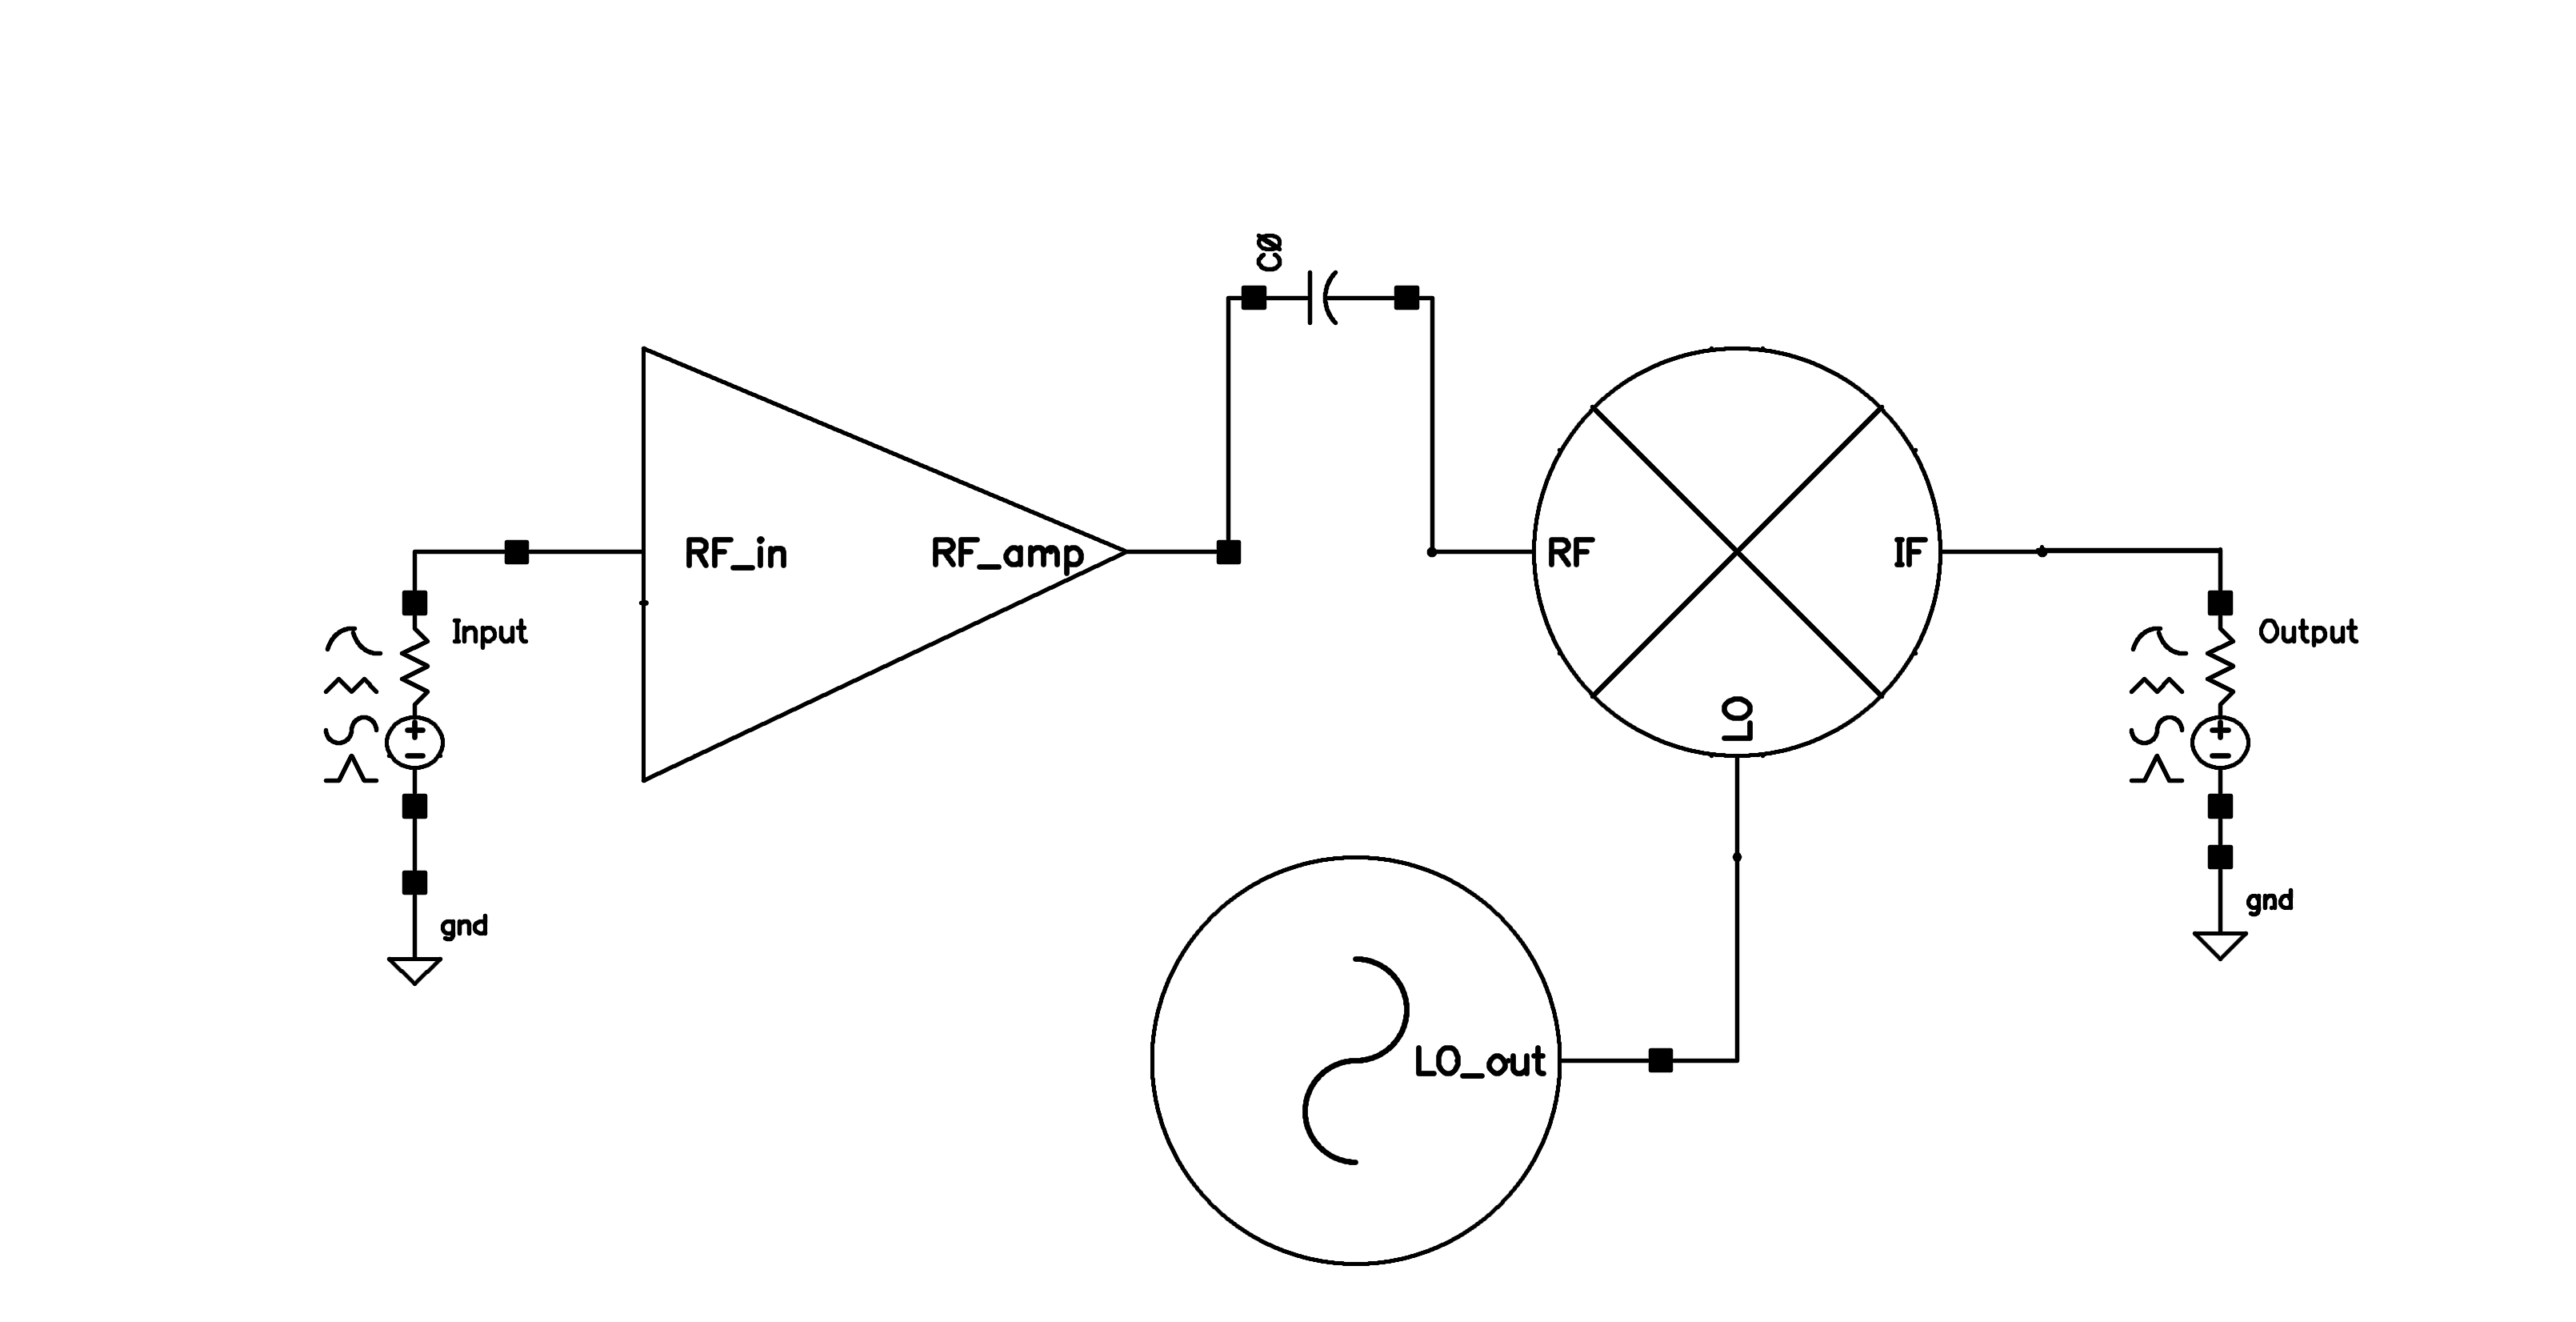
\includegraphics[width=0.5\textwidth]{figures/FullSystem.png}
    \caption{Full system circuit integration, with LNA, Mixer, and VCO. Coupling capacitor removes DC offset from LNA. }
    \label{fig:fullsystem}
\end{figure}

In order to test the system, a transient analysis was preformed with an initial input signal of 1 mV at 403.5 MHz. Fig.~\ref{fig:fullsystemtrans} shows a clean output response from the system that swings from 55 mV to -70 mV at 3.5 MHz. This leads to an overall swing of 62.5 mV, therefore the conversion gain of the entire system is $20log(\frac{62.5 mV}{1 mV})$ or {\bf 35.92 dB}.

\begin{figure}[h]
   \centering
    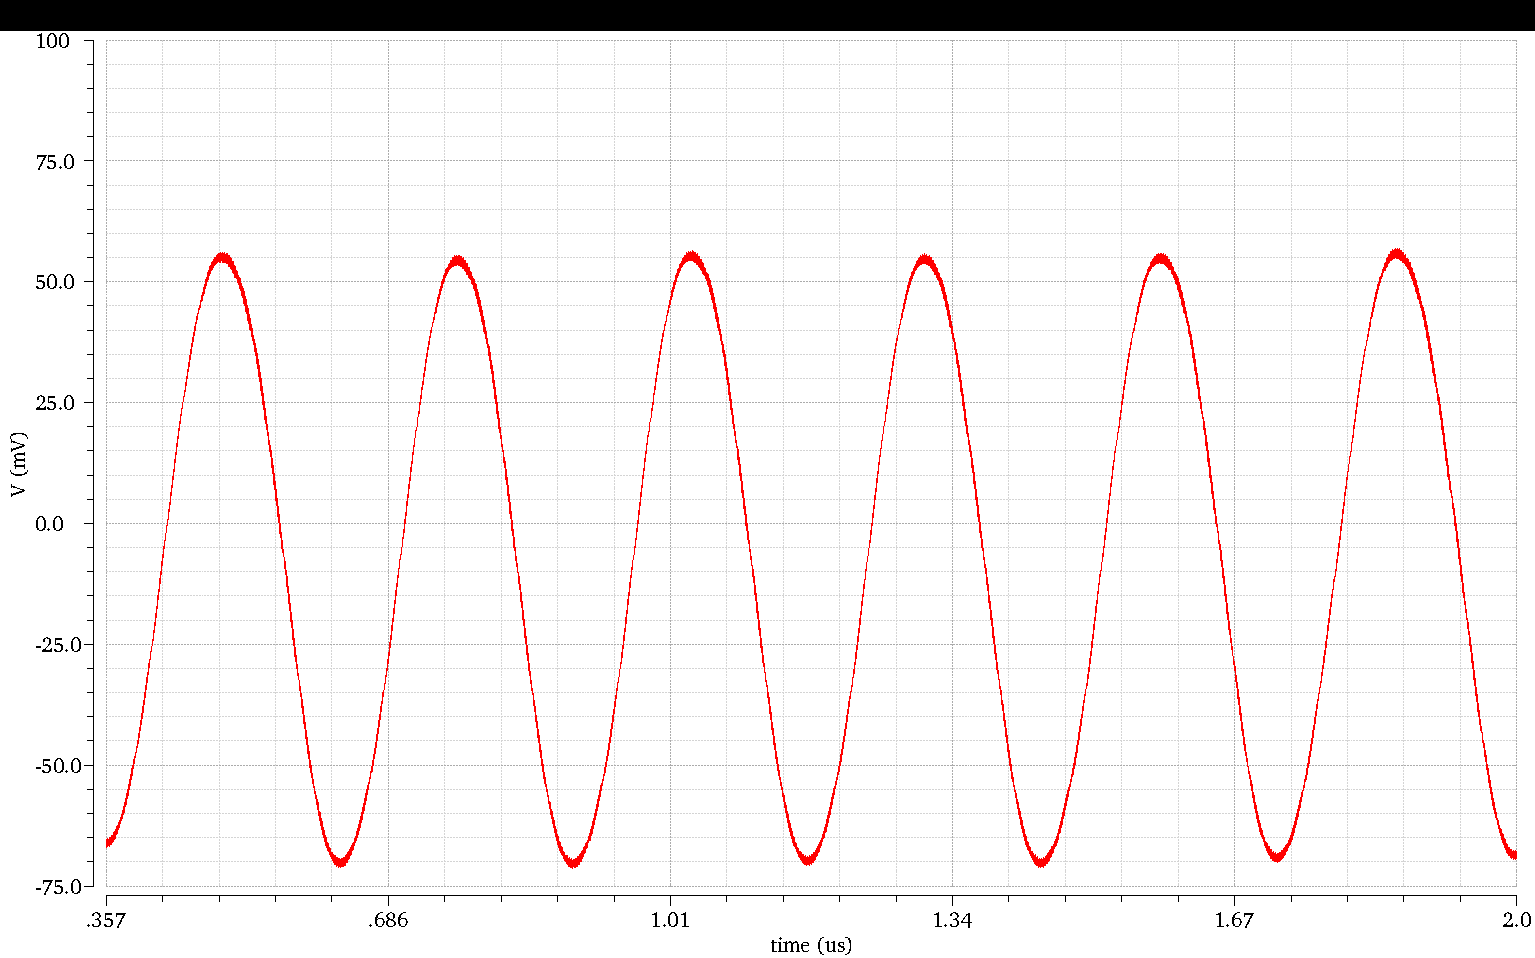
\includegraphics[width=0.5\textwidth]{figures/FullSystemTrans}
    \caption{Transient response of receiver after 357ns startup time.}
    \label{fig:fullsystemtrans}
\end{figure}

In order to measure the Noise Figure, the VCO was removed and an ideal source was used instead. Although the oscillator in theory would contribute slightly to the noise, it was determined that due to its low LO-IF feed-through that the oscillator has a negligible effect to the total noise. Fig.~\ref{fig:fullsystemnoise} shows the total noise of the system, at the corner frequency of the output, it was determined that the total noise was {\bf 3.65 dB}.

\begin{figure}[h]
   \centering
    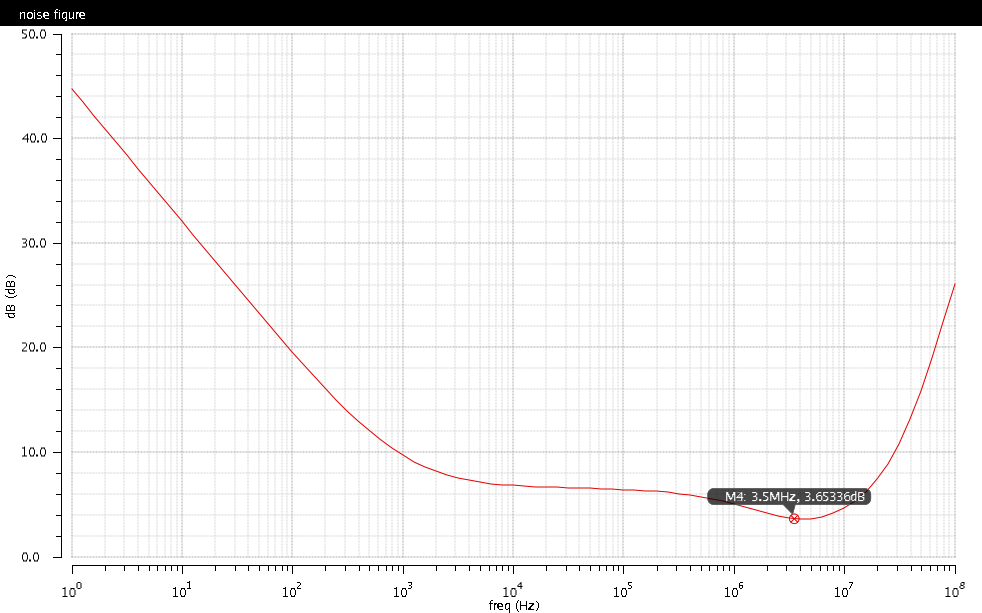
\includegraphics[width=0.5\textwidth]{figures/FullSysNoiseFigure.png}
    \caption{Full system noise due to LNA and Mixer.}
    \label{fig:fullsystemnoise}
\end{figure}

The overall linearity of the system is about {\bf -31 dBm} however a graph is not shown due to technical issues with the Cadence software. Overall the full system results can be found in TABLE ~\ref{tab:systemresults}.


\begin{table}[H]
\caption{Final results from system integration.}
\label{tab:systemresults}
\begin{center}
	\begin{tabular}{ c | c  }

  		Conversion Gain & 35.92 dB \\ \hline
  		Noise Figure & 3.65 dB \\ \hline
  		IIP3 & -31 dBm\\ \hline
		Power & 1.8 mW \\

	\end{tabular}

\end{center}

\end{table}

\section{Conclusions}
Conclusions go here




\bibliographystyle{ieeetran}
\bibliography{references}


\end{document}


